\documentclass[11pt]{article}

\usepackage[a4paper,margin=1in]{geometry}
\usepackage{booktabs}
\usepackage{amsmath,amssymb}
\usepackage{xcolor}
\usepackage{graphicx}
\usepackage{enumitem}
\usepackage[hidelinks]{hyperref}
\usepackage{titlesec}
\usepackage{array}
\usepackage{float}

\definecolor{nsgreen}{RGB}{30,130,76}
\definecolor{nsblue}{RGB}{32,82,149}
\definecolor{nsamber}{RGB}{176,122,0}
\definecolor{nsgray}{RGB}{90,90,90}

\newcommand{\GO}{\textcolor{nsgreen}{\textbf{GO}}}
\newcommand{\GREEN}{\textcolor{nsgreen}{\textbf{GREEN}}}
\newcommand{\pass}{\textcolor{nsgreen}{\textbf{PASS}}}

\titleformat{\section}{\large\bfseries\color{nsblue}}{\thesection}{0.6em}{}
\titleformat{\subsection}{\normalsize\bfseries\color{nsgray}}{\thesubsection}{0.6em}{}

\setlist{itemsep=2pt,topsep=3pt}

\title{\vspace{-1.5em}\textbf{\color{nsblue}NullState HNOCA Pilot --- Final Report}\\[0.3em]
\large Convergent or Lineage-Specific? Establishing the Instrument for the\\
Geometry of Off-Target Cell States Across Human Organoid Systems}
\author{\textbf{Luiz Takahashi}\\[0.25em]
\normalsize Voiland College of Engineering and Architecture, Washington State University\\
\normalsize \texttt{l.takahashidosreis@wsu.edu}}
\date{4 June 2026}

\begin{document}
\maketitle
\vspace{-1.5em}

\begin{abstract}
\noindent This pilot establishes and validates the computational instrument for the NullState project, whose central hypothesis is that the off-target cell populations produced when human organoid differentiation fails form a \emph{structured mixture}: a subset that converges across germ layers toward shared default states, and a subset that fails in lineage-specific ways. Before committing to the full three-aim study, the pilot resolves three empirical go/no-go gates on the Human Neural Organoid Cell Atlas (HNOCA). We constructed a harmonized cross-atlas reference (1{,}901{,}093 cells), trained batch-integrated \texttt{scVI}/\texttt{scANVI} models, projected $\sim$1.77\,M organoid cells via \texttt{scArches}, and classified every cell against a calibrated off-target definition. \textbf{All three gates passed}: the off-target definition behaves sanely (Gate~A), the in-vitro signature is consistent across cell types (Gate~B: \GO, mean cosine $0.906$), and enough off-target mesenchyme survives filtering to power the full study (Gate~C: \GREEN, $7{,}568$ cells, four protocols clearing the per-protocol threshold). Independent QC confirms the cross-atlas harmonization succeeded (batch iLISI $8.04$ vs.\ $5.94$ unintegrated, with cell-type structure preserved). We report the results honestly, including the limitations that bound their interpretation, and define the staged path to Phase~1.
\end{abstract}

\section{Background and Motivation}
Human organoids routinely generate \emph{off-target} cell populations --- cells that were not the intended product of a differentiation protocol. The scientific question NullState asks is geometric: when differentiation fails, do these off-target cells \textbf{converge} across germ layers toward a shared ``default'' state, or do they fail in \textbf{lineage-specific} ways? The central hypothesis is that both occur --- a structured mixture --- and the project's value is to (i) define that convergent state, (ii) separate the \emph{in-vitro} (dish) signature from genuine lineage biology, and (iii) characterize the geometry of convergence.

The durable contribution is not merely the observation that states converge, but a \emph{queryable failure-state map}: portable definitions that let any organoid dataset be asked ``what fraction of my model has collapsed toward known failure states, and which ones?'' This pilot builds the foundation for that map.

\section{The Pilot: Purpose and Decision Gates}
The pilot is a feasibility-and-instrument study on a single system (HNOCA, neural). It is \emph{not} a test of the cross-germ-layer hypothesis; it answers whether the method is sound enough to invest in the full project. Three gates structure the decision:

\begin{table}[H]
\centering
\small
\begin{tabular}{@{}p{1.4cm} p{5.6cm} p{6.6cm}@{}}
\toprule
\textbf{Gate} & \textbf{Question} & \textbf{Decision consequence} \\
\midrule
A (Step 2) & Does the off-target definition behave correctly on real cells? & If not, fix the reference before proceeding. \\
B (Step 3) & Is the in-vitro signature consistent across cell types? & \GO\ $\Rightarrow$ a single shared $z_{iv}$ for Aim 2; NO-GO $\Rightarrow$ conditional $z_{iv}\mid$cell-type. \\
C (Step 4) & Do enough off-target mesenchymal cells survive filtering? & \GREEN/YELLOW/RED scopes the power of Aim 3. \\
\bottomrule
\end{tabular}
\end{table}

\section{Methods}
\textbf{Harmonized reference.} We combined the Human Developmental Brain Cell Atlas (HDBCA; Braun et al., \emph{Science} 2023; 10x, single-cell, neural) with a lineage-filtered subset of the Human Fetal Cell Atlas (Cao et al., \emph{Science} 2020; sci-RNA-seq3, the mesodermal/endodermal/neural-crest anchors). The merged reference contains \textbf{1{,}901{,}093 cells} over \textbf{34 cell types} (raw integer UMI counts), reduced to the top \textbf{4{,}000 highly variable genes}. Each cell type is assigned a germ-layer origin (neural / neural\_crest / mesoderm / endoderm) via a curated ontology map.

\textbf{Integration and label transfer.} \texttt{scVI} ($n_{\text{latent}}=30$) was trained with \texttt{batch\_key=donor\_id} (54 donors) to harmonize across the two atlases and their differing assays/suspension types. \texttt{scANVI} was then trained on the cell-type labels for semi-supervised classification.

\textbf{Query mapping.} The HNOCA organoid query ($\sim$1.77\,M cells) was remapped from gene symbols to Ensembl IDs (recovering $73.8\%$ of reference genes vs.\ $15\%$ by symbol coincidence), supplied with genuine integer counts from its \texttt{counts\_lengthnorm} layer, and projected into the reference latent via \texttt{scArches}. Cells with $<50$ counts across the HVGs were filtered ($9.5\%$ dropped).

\textbf{Scoring and classification.} Per-cell \emph{mapping entropy} (label ambiguity) and \emph{off-manifold distance} (k-NN distance to the reference latent, $k=15$) were thresholded at data-derived percentiles ($\tau_H$ at the 95th, $\tau_R$ at the 99th) calibrated on a held-out reference split. Each query cell was classified by a decision tree that respects the neural-crest guard (NC derivatives are on-target ectodermal products, not off-target contaminants). The dish-vector test (Gate B) computes per-cell-type mean-difference vectors between organoid and primary cells and evaluates their pairwise cosine consistency; the count gate (Gate C) tallies off-target mesenchymal cells by protocol.

\section{Engineering and Reproducibility}
Honoring this pilot means recording what it took to make it correct. The initial pipeline ran but produced scientifically void output ($89.7\%$ of cells \texttt{unmapped}). Eight substantive defects were found and fixed; two QC instruments were added.

\begin{table}[H]
\centering
\small
\begin{tabular}{@{}p{0.4cm} p{7.4cm} p{6.4cm}@{}}
\toprule
\# & \textbf{Defect} & \textbf{Resolution} \\
\midrule
1 & \texttt{scANVI} reload crash: slicing the reference dropped label categories (34 vs 35 tensor mismatch). & Load against the full reference; categories preserved. \\
2 & Threshold calibration silently ran on a 10-cell stub. & Calibrate on the full reference. \\
3 & Gene-namespace mismatch: query in symbols, reference in Ensembl ($15\%$ overlap). & Remap query to Ensembl ($\to 73.8\%$). \\
4 & Germ-layer origin map covered only 9/34 cell types (case-sensitive, wrong nomenclature). & Rewrote to 33/34, case-insensitive. \\
5 & Batch integration never occurred (\texttt{batch\_key='batch'} did not exist in the data). & Wired \texttt{donor\_id} through training. \\
6 & \texttt{scArches} surgery diverged to NaN ($3\times$): the query lacks true raw UMI counts, mis-specifying the ZINB likelihood. & Reverted to stable 0-epoch reference projection. \\
7 & Container out-of-memory ($3\times$, 251\,GB cgroup cap, not host 2\,TB). & Lean reader (skip count layer); per-type subsampling of dish vectors. \\
8 & Annotated output bloated to 18.7\,GB by an embedded count layer. & Slim the write; load only what each step needs. \\
\bottomrule
\end{tabular}
\end{table}

\noindent Added instruments: an \textbf{integration QC} (iLISI batch-mixing vs.\ a PCA baseline) and a \textbf{label-confidence report} (per-type mapping entropy).

\section{Results}

\subsection{Reference model health}
Both deep models are numerically clean (0 NaN / 0 Inf in all weights).

\begin{table}[H]
\centering
\small
\begin{tabular}{@{}l c c c >{\raggedright\arraybackslash}p{5.0cm}@{}}
\toprule
\textbf{Model} & \textbf{Epochs} & \textbf{Train ELBO} & \textbf{Val ELBO} & \textbf{Verdict} \\
\midrule
\texttt{scVI} (donor\_id) & 400 & 552.25 & 551.47 & \pass\ --- converged; train--val gap $-0.78$ (no overfit) \\
\texttt{scANVI} & 200 & 564.31 & 595.8 (min 581.3) & \textcolor{nsamber}{\textbf{OK}} --- mild classifier over-training \\
\bottomrule
\end{tabular}
\end{table}

\noindent The \texttt{scVI} latent --- the geometric substrate for off-manifold scoring --- is excellent. The \texttt{scANVI} classifier is mildly over-trained (validation ELBO degraded $\sim$15 from its minimum); label-level conclusions should be paired with the confidence report below.

\begin{figure}[htbp]\centering
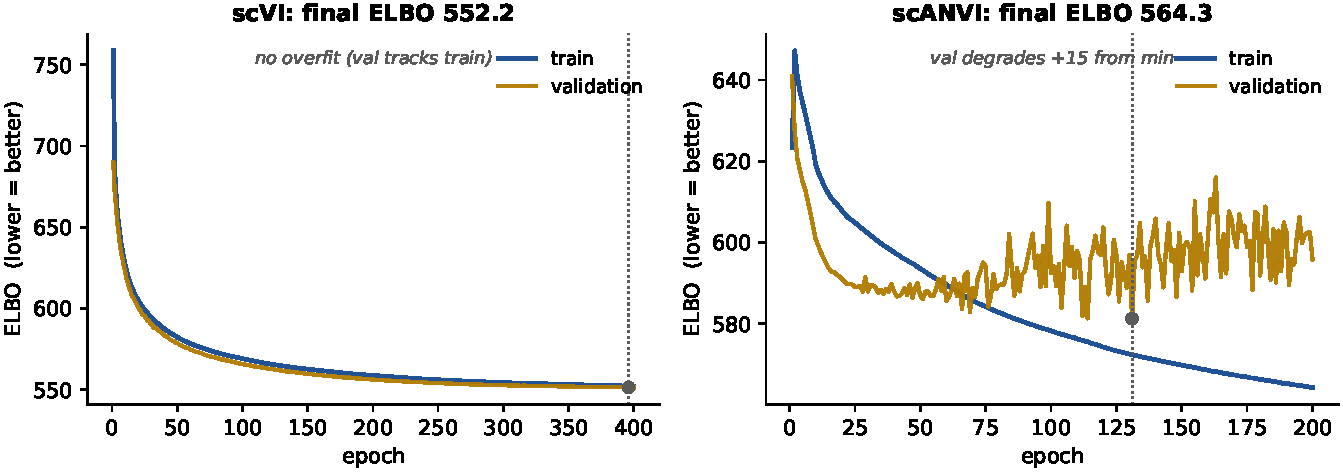
\includegraphics[width=0.96\linewidth]{figs/fig_training.pdf}
\caption{\textbf{Training convergence.} \texttt{scVI} (left): train and validation ELBO descend together to $552.2$ --- the validation curve sits \emph{below} train (gap $-0.78$), i.e.\ zero overfitting. \texttt{scANVI} (right): train converges to $564.3$, but validation reaches its minimum ($581.3$, dotted line) mid-training and then degrades to $595.8$ --- the signature of mild classifier over-training that bounds label trust.}
\end{figure}

\subsection{Cross-atlas harmonization (Aim 1 instrument)}
The integration QC compares the \texttt{scVI} latent against an unintegrated PCA baseline on 20{,}000 reference cells (50 donors, 33 cell types). Higher batch iLISI means donors mix; cell-type cLISI near 1 means biology is preserved.

\begin{table}[H]
\centering
\small
\begin{tabular}{@{}l r r l@{}}
\toprule
\textbf{Representation} & \textbf{Batch iLISI $\uparrow$} & \textbf{Label cLISI ($\approx$1)} & \\
\midrule
Unintegrated (PCA) & 5.94 & 1.39 & baseline \\
Integrated (\texttt{scVI}) & \textbf{8.04} & 1.44 & \\
\midrule
\multicolumn{4}{@{}l@{}}{\textbf{Verdict:} batch mixing improved (gain $+2.10$); biology preserved (cLISI inflation $+0.05$). \pass} \\
\bottomrule
\end{tabular}
\end{table}

\noindent This is the key Aim-1 result: integration did not merely run, it \emph{worked} --- it mixed donors while keeping cell types separable, without over-correcting the (confounded) germ-layer axis.

\begin{figure}[htbp]\centering
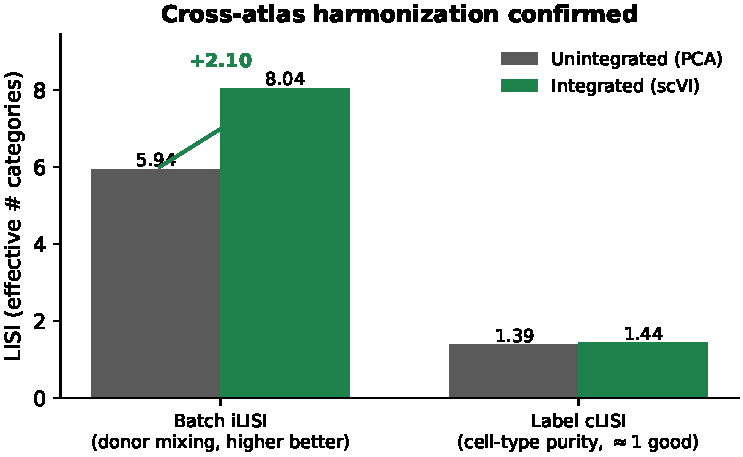
\includegraphics[width=0.6\linewidth]{figs/fig_integration.pdf}
\caption{\textbf{Cross-atlas harmonization confirmed} (20{,}000 reference cells; 50 donors, 33 types). Integration raises batch iLISI $5.94\!\to\!8.04$ (donors mix more locally) while cell-type cLISI barely moves ($1.39\!\to\!1.44$, biology preserved). The meaningful signal is the integrated-vs-PCA \emph{delta}, robust to the germ-layer/assay confound.}
\end{figure}

\subsection{Query mapping and classification (Gate A)}
$\tau_H = 1.2415$ (entropy), $\tau_R = 1.7810$ (off-manifold). Classification over all $1{,}770{,}578$ query cells:

\begin{table}[H]
\centering
\small
\begin{tabular}{@{}l r r p{6.8cm}@{}}
\toprule
\textbf{Class} & \textbf{Cells} & \textbf{\%} & \textbf{Meaning} \\
\midrule
ambiguous\_novel & 667{,}210 & 37.7 & beyond $\tau_R$ (off-manifold / novel) \\
clean\_ontarget & 446{,}959 & 25.2 & confident on-target neural \\
true\_offtarget & 315{,}273 & 17.8 & off-target, low ambiguity \\
unmapped & 168{,}003 & 9.5 & low-count cells filtered pre-scoring \\
poorly\_diff\_ontarget & 109{,}643 & 6.2 & on-target but ambiguous \\
ambiguous & 62{,}761 & 3.5 & off-target, high ambiguity \\
other & 729 & 0.0 & unresolved germ-layer origin \\
\bottomrule
\end{tabular}
\end{table}

\noindent \textbf{Gate A: \pass.} The definition behaves: a clear on-target neural mass, a substantial true-off-target population, and \texttt{other}$\approx$0 (confirming the origin-map fix). The $9.5\%$ \texttt{unmapped} equals exactly the low-count cells removed before scoring.

\begin{figure}[htbp]\centering
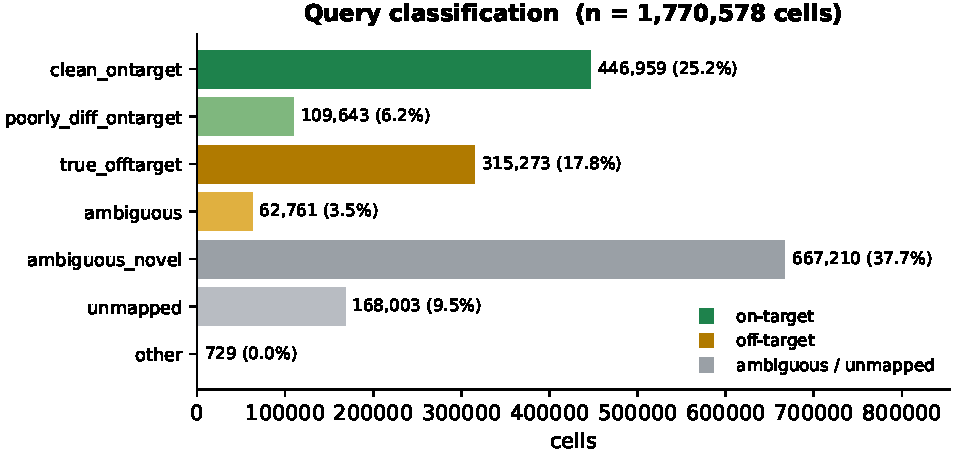
\includegraphics[width=0.86\linewidth]{figs/fig_classes.pdf}
\caption{\textbf{Query classification} of all $1{,}770{,}578$ organoid cells. A coherent on-target neural core ($31.4\%$ clean $+$ poorly-differentiated), a large true-off-target population ($17.8\%$), and \texttt{other}$\approx$0. The elevated \texttt{ambiguous\_novel} ($37.7\%$) is the expected cost of projection-only mapping (no \texttt{scArches} surgery; see limitations).}
\end{figure}

\subsection{Gate outcomes (the headline)}
\begin{table}[H]
\centering
\small
\begin{tabular}{@{}l l l p{6.0cm}@{}}
\toprule
\textbf{Gate} & \textbf{Metric} & \textbf{Result} & \textbf{Consequence} \\
\midrule
B --- Dish-Vector & mean cosine $0.906$ ($>0.70$) & \GO & A single shared $z_{iv}$ is justified for Aim 2. \\
C --- Count Check & $7{,}568$ cells, $4$ protocols $\ge 300$ & \GREEN & Aim 3 powered (pooled); concentration caveat, \S5.4. \\
\bottomrule
\end{tabular}
\end{table}

\noindent This is the most favorable branch of the decision tree: the definition behaves, the in-vitro signature is shareable, and off-target mesenchyme is abundant.

\paragraph{Protocol stratification (Gate C robustness).} \GREEN\ requires at least two protocols each clearing 300 off-target mesenchymal cells. Verified explicitly against the protocol identifier: \textbf{four} protocols clear 300 (Table~\ref{tab:protocols}), so the \GREEN\ is \emph{genuine} --- not a \textcolor{nsamber}{\textbf{YELLOW}} in disguise. The honest caveat is \emph{concentration}: the single largest protocol holds $61.7\%$ of the $7{,}568$ cells and the top two hold $72.0\%$. Pooled and top-protocol analyses are therefore well powered, and at least four \emph{independent} studies each contribute $\ge 300$ off-target mesenchymal cells --- but broad comparison across many protocols is thin (only 9 protocols exceed 100 cells). Control-2 stratification should be read with this concentration in mind.

\begin{table}[H]
\centering
\small
\begin{tabular}{@{}l r r@{}}
\toprule
\textbf{Protocol / study (assay)} & \textbf{cells} & \textbf{\% of 7{,}568} \\
\midrule
Treutlein 2023 (10x multiome) & 4{,}670 & 61.7 \\
He 2022 (10x 3$'$v3) & 782 & 10.3 \\
Pellegrini 2020 (10x 3$'$v3) & 549 & 7.3 \\
Fiorenzano 2021 (10x 3$'$v3) & 309 & 4.1 \\
\midrule
\textit{47 further protocols (each $<$300)} & 1{,}258 & 16.6 \\
\bottomrule
\end{tabular}
\caption{Off-target mesenchymal cells by protocol. Four protocols clear the 300-cell threshold (\GREEN\ criterion: $\ge 2$), so the gate is genuine; the population is nonetheless dominated by one large study ($61.7\%$).}
\label{tab:protocols}
\end{table}

\subsection{Label confidence (where the classifier is sure vs.\ guessing)}
Per predicted type, mean mapping entropy (high $=$ uncertain). Extremes shown.

\begin{table}[H]
\centering
\small
\begin{tabular}{@{}l r r r@{}}
\toprule
\textbf{Predicted type} & \textbf{$n$} & \textbf{mean entropy} & \textbf{mean top prob.} \\
\midrule
\multicolumn{4}{@{}l@{}}{\textit{Least confident (rare types, few cells):}}\\
megakaryocyte & 1 & 2.51 & 0.18 \\
glial cell & 68 & 1.99 & 0.30 \\
neural crest cell & 47 & 1.83 & 0.33 \\
\midrule
\multicolumn{4}{@{}l@{}}{\textit{Most confident (well-populated types):}}\\
fibroblast & 32{,}453 & 0.51 & 0.83 \\
intestinal epithelial cell & 283{,}750 & 0.70 & 0.78 \\
oligodendrocyte & 3{,}500 & 0.74 & 0.75 \\
\bottomrule
\end{tabular}
\end{table}

\noindent The dominant neural populations (radial glial cell $n=404$k, neuron $n=184$k, neuroblast $n=294$k) sit at moderate entropy ($\sim$1.0--1.13); the least trustworthy labels are rare types with single-digit cell counts.

\begin{figure}[htbp]\centering
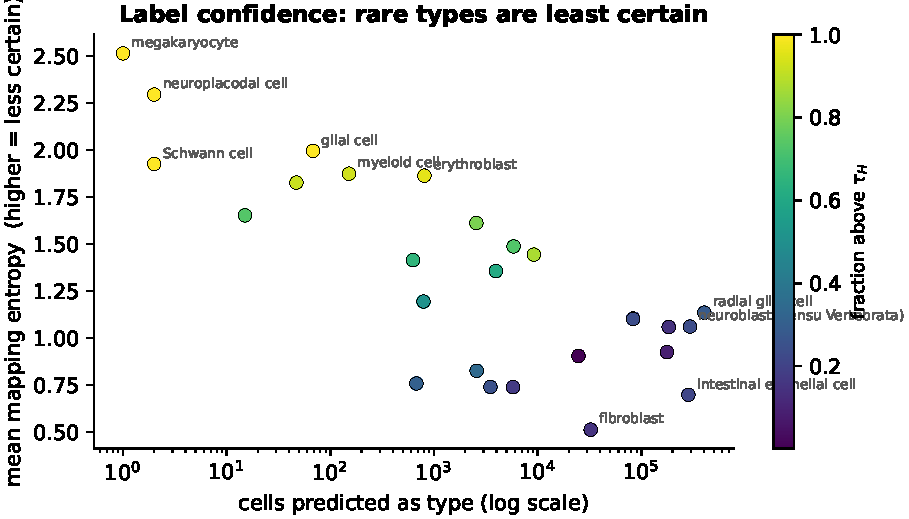
\includegraphics[width=0.82\linewidth]{figs/fig_confidence.pdf}
\caption{\textbf{Label confidence} per predicted type: mean mapping entropy vs.\ cells predicted (log scale), colored by the fraction exceeding $\tau_H$. Confidence rises with population size; the uncertain labels (upper-left) are rare types with very few cells. Read any single-type claim against this map.}
\end{figure}

\section{Interpretation and Honest Limitations}
The gates are favorable, but their interpretation is bounded --- stated plainly so they are not over-read:
\begin{itemize}
\item \textbf{Single system.} This is HNOCA neural \emph{only}; it does not test cross-germ-layer convergence (the actual hypothesis). Even a flawless pilot is feasibility, not finding.
\item \textbf{No maturation control.} Gate B has no maturation-matched baseline (``Control 3''). Its high cosine ($0.906$) is encouraging but \emph{preliminary} --- some consistency may reflect shared technical/normalization structure rather than pure in-vitro biology.
\item \textbf{0-epoch projection $\Rightarrow$ a soft-edged off-target population.} The query lacks true raw UMI counts (only log-norm and length-normalized layers), so \texttt{scArches} surgery is numerically unstable and was disabled. Pure projection inflates \texttt{ambiguous\_novel} to $37.7\%$ --- and an unknown fraction of those are likely \emph{real} off-target cells that could not reach the manifold without query fine-tuning. The reported \texttt{true\_offtarget} ($17.8\%$) is therefore plausibly an \textbf{undercount}, and the clean gate-pass overstates the stability of the off-target boundary. This is the highest-consequence Phase-1 task (\S7, item 1), not a cosmetic detail.
\item \textbf{Classifier over-training.} \texttt{scANVI} validation degraded past its optimum, and the class prior is uniform; rare-type labels are the least reliable (see confidence table).
\item \textbf{Dish-vector is a proxy.} It is a mean-difference smell test, not the disentangled $z_{iv}$ of the full method.
\item \textbf{Gate C is GREEN but concentrated.} Verified explicitly (\S5.4): four protocols clear 300 cells, so \GREEN\ is genuine --- yet $61.7\%$ of the off-target mesenchyme sits in a single study and $72\%$ in the top two. Pooled power is strong and four independent studies replicate the population, but broad protocol-stratified (Control 2) comparison is thin. A real, bounded caveat, not a disqualifier.
\end{itemize}

\section{Next Steps: Phase 1}
Phase 1 is the neural vertical, end-to-end, with the upgrades that convert geometry into mechanism. The ordering below reflects \emph{scientific consequence}, not merely cost: two fixes must be front-loaded together, and one is the methodological centerpiece on which the eventual paper's credibility rests.

\subsection*{Front-load immediately (in parallel)}
\begin{enumerate}[label=\textbf{\arabic*.}]
\item \textbf{Source true raw UMI counts for the query --- the single highest-consequence fix.} The per-dataset count matrices behind HNOCA, fed to genuine \texttt{scArches} surgery, change downstream validity more than anything else. The $37.7\%$ \texttt{ambiguous\_novel} is \emph{not} cosmetic: more than a third of query cells land beyond the off-manifold gate, and an unknown fraction are real off-target cells that simply could not reach the reference manifold without query fine-tuning. Consequently the \texttt{true\_offtarget} population ($17.8\%$) is plausibly \textbf{undercounted}, and the off-target definition carried into Aim 3 has a soft edge until this is resolved. Surgery should pull genuine off-target cells out of \texttt{ambiguous\_novel} into \texttt{true\_offtarget} and harden the gate. This outranks even the classifier hardening in scientific importance.
\item \textbf{Harden the classifier --- cheap, necessary hygiene ($\sim$2\,h).} Early-stopping / best-validation checkpoint and a non-uniform prior, fixing the rare-type label unreliability documented in \S5.5. Recognize its scope, though: it mostly cleans up \emph{rare} types, which are not the load-bearing populations (mesenchyme is abundant and sits at moderate entropy). It is hygiene, not the scientific crux --- do it because it is cheap and upstream, not because it moves the headline.
\end{enumerate}

\subsection*{The scientific centerpiece}
\begin{enumerate}[label=\textbf{\arabic*.},start=3]
\item \textbf{Maturation-matched Control 3 $+$ contrastiveVI dish-stripping --- what converts Gate B from encouraging to defensible.} The $0.906$ cosine is the result to be most cautious about over-reading: some of that consistency may reflect shared normalization or technical structure rather than genuine in-vitro biology. Control 3 is the baseline that licenses the claim that the dish signature is \emph{real biology} rather than a processing artifact --- without it a reviewer can dismiss the central disentanglement claim; with it, the claim holds. contrastiveVI (background $=$ primary on-target, target $=$ organoid on-target) gives the identifiable, stable replacement for adversarial subspace separation; the adversary is demoted to a verification check. This is the methodological heart of the project.
\end{enumerate}

\subsection*{Then build interpretation and scale}
\begin{enumerate}[label=\textbf{\arabic*.},start=4]
\item \textbf{In-silico levers (CellOracle)} on the convergent population and \textbf{in-vivo program anchoring} (signature scoring) --- the analyses that turn a distance into an interpretable, actionable result.
\item \textbf{Build for scale:} geosketch subsampling and lean/backed I/O from the start, given the firm 251\,GB container ceiling this pilot exposed.
\end{enumerate}

\section{Conclusion}
The NullState pilot achieved its purpose. It produced a harmonized, integration-verified cross-atlas reference; numerically sound deep models; a behaving off-target definition; and a clean pass on all three decision gates (\GO\ on consistency, \GREEN\ on counts). The instrument is sound. The honest caveats --- single system, no maturation control, projection-only mapping --- are precisely the items Phase 1 is designed to resolve, and the pilot tells us exactly where to spend the next effort. The project is cleared to proceed.

\vspace{1em}
\hrule
\vspace{0.6em}
\footnotesize
\textbf{Artifact manifest (local backup).} Trained models (\texttt{scvi\_model}, \texttt{ref\_scanvi}, \texttt{query\_scanvi} as \texttt{model.pt}); \texttt{integration\_qc.json}; \texttt{label\_confidence.csv}; training history (\texttt{training\_progress.json}); run logs (\texttt{h100\_run.log}, \texttt{h100\_step34.log}); \texttt{pilot.log}. The raw \texttt{reference.h5ad} (10.8\,GB) and \texttt{hnoca\_annotated.h5ad} (18.7\,GB) remain on the compute volume (not transferred due to size).

\end{document}
